\subsubsection{\textit{World service}}
\label{sec:world-service}

El \textit{world service} es el encargado de gestionar los mundos y sus zonas, así como la orquestación de los
servidores de juego asociados a cada una de ellas. El servicio se divide en tres componentes principales: la
gestión de mundos, la gestión de zonas y el registro de servidores.
\vspace{0.25cm}

Un mundo se crea mediante \texttt{POST /world}, donde el usuario proporciona un nombre, una descripción y los
datos de configuración del mundo en formato JSON. Esto proporciona un ID al mundo en los datos del mundo 
(\textit{world data}), con el cual se puede actualizar el mundo ya creado con
\texttt{PUT /world/\{id\}}. Adicionalmente, mundo almacena además un campo \texttt{createable\_data}, que contiene la 
configuración de los objetos que pueden ser instanciados en él y que puede actualizarse de forma independiente mediante
\texttt{PUT /world/\{id\}/createable-data}.
\vspace{0.25cm}

La consulta de un mundo se realiza mediante \texttt{GET /world/\{id\}}, que retorna la configuración completa
junto con los metadatos de sus zonas. El listado de mundos se obtiene mediante \texttt{GET /world}, que admite
paginación y busqueda por filtros utilizando los parámetros \texttt{offset}, \texttt{limit} y \texttt{user\_id}, 
este último en caso de querer buscar un mundo bajo el creado del mundo. 

\vspace{0.25cm}

Cada mundo se divide en zonas, identificadas por un número entero positivo. Una zona se publica o actualiza
mediante \texttt{PUT /world/\{id\}/zones/\{zone\_id\}}, operación que requiere que el usuario sea propietario
del mundo. Cada zona almacena sus propios datos de configuración en formato JSON y expone dos indicadores de
estado: \texttt{is\_active}, que indica si la zona tiene un servidor de juego asignado, e \texttt{is\_online},
que indica si dicho servidor está en ejecución en ese momento.
\vspace{0.25cm}

\begin{figure}[H]
    \centering
    \begin{adjustbox}{width=1.10\textwidth, center}
        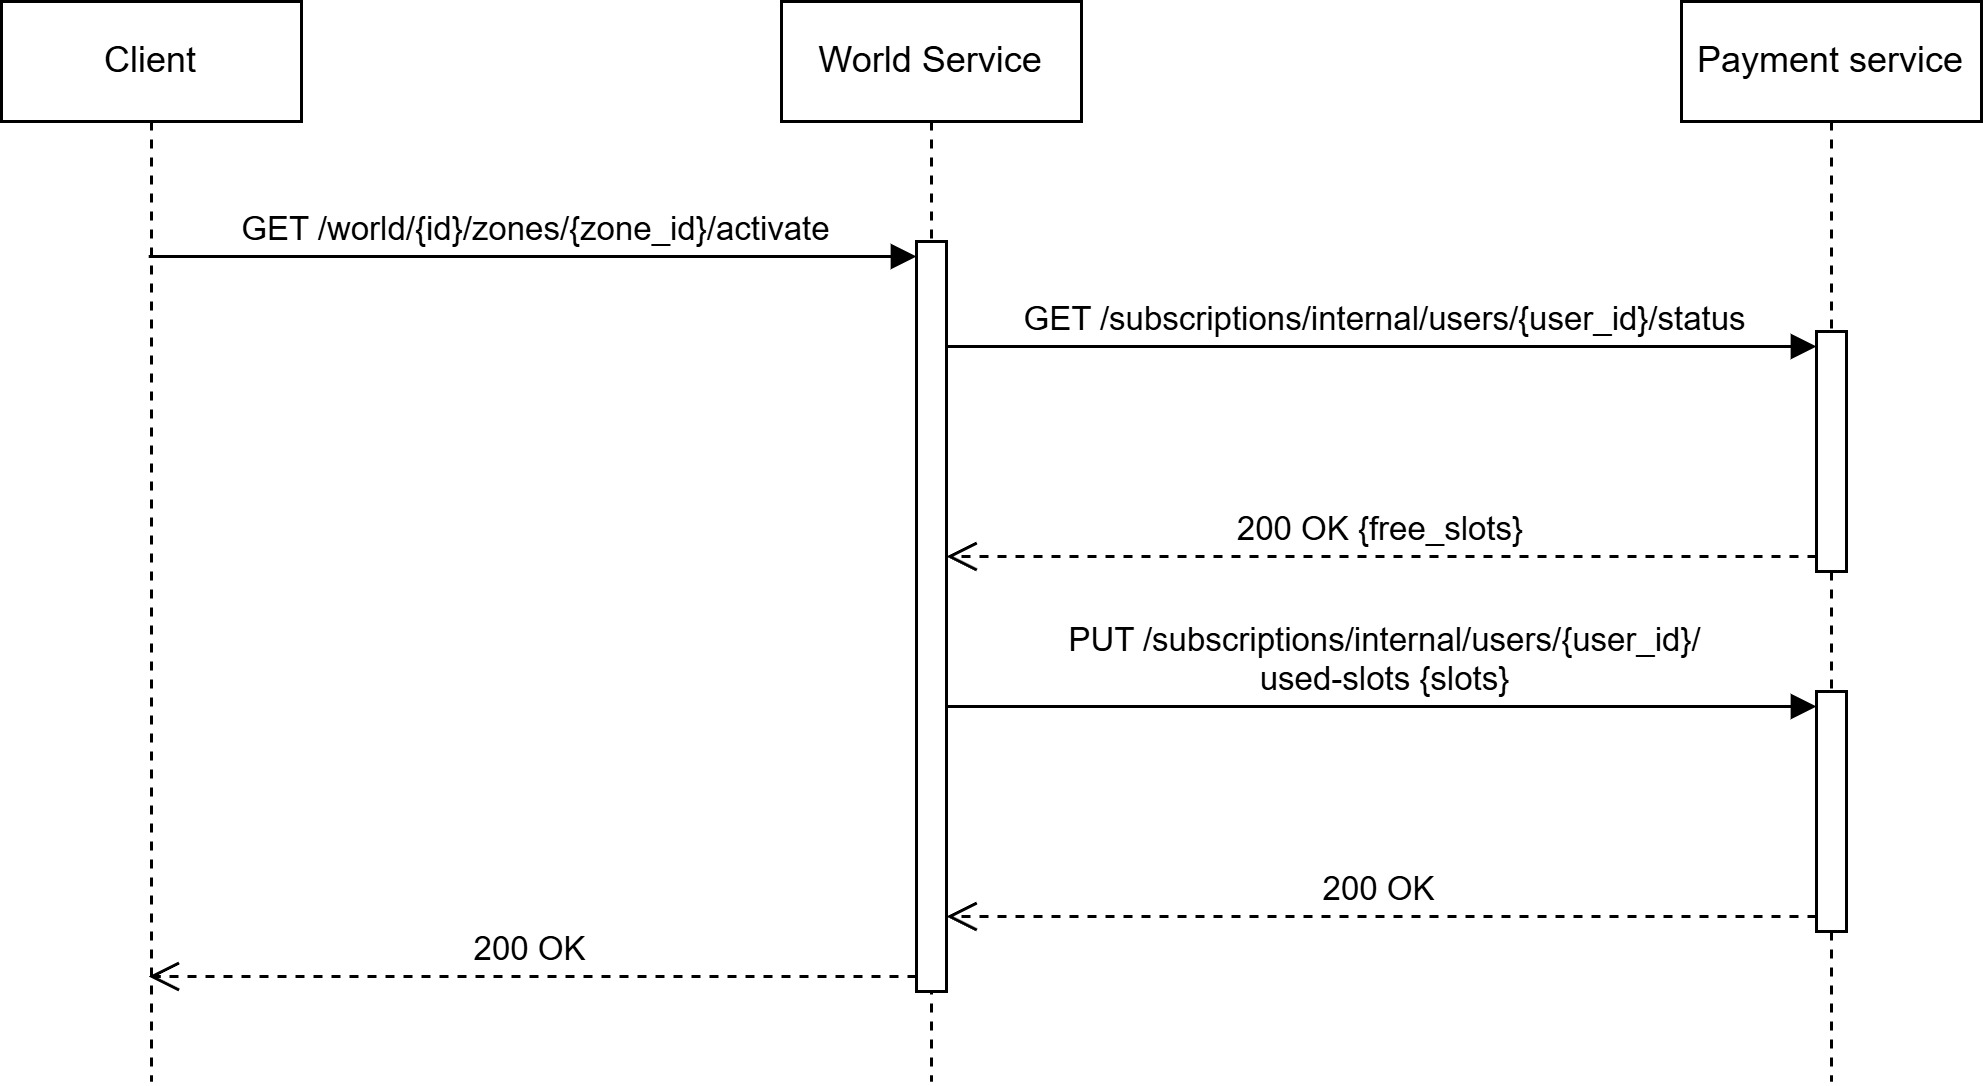
\includegraphics{img/09-technical-details/core-service/world-service-case-1.jpg}
    \end{adjustbox}
    \caption{Diagrama de secuencia del consumo de un \textit{slot}.}    \label{fig:world-service-case-1}
\end{figure}

La activación de una zona se realiza mediante \texttt{GET /world/\{id\}/zones/\{zone\_id\}/activate}, que
verifica la propiedad del mundo, consume un \textit{slot} de la suscripción del usuario e inicia el proceso de
orquestación del servidor correspondiente. La desactivación se realiza de forma análoga mediante
\texttt{GET /world/\{id\}/zones/\{zone\_id\}/deactivate}, que detiene el servidor y libera el \textit{slot}
consumido. El consumo de esos \textit{slots} es chequeado por \texttt{GET /subscriptions/internal/users/} 
\texttt{\{user\_id\}/status} y consumido finalmente por \texttt{PUT /subscriptions/internal/users/\{user\_id\}/} 
\texttt{used-slots} del \textit{payment service}. Existe además un \textit{endpoint} interno \texttt{GET /world/internal/users/}
\texttt{\{user\_id\}/stop-jobs} que detiene todas las zonas activas de un usuario, utilizado por el \textit{payment service} cuando 
se cancela una suscripción.
\vspace{0.25cm}

\begin{figure}[H]
    \centering
    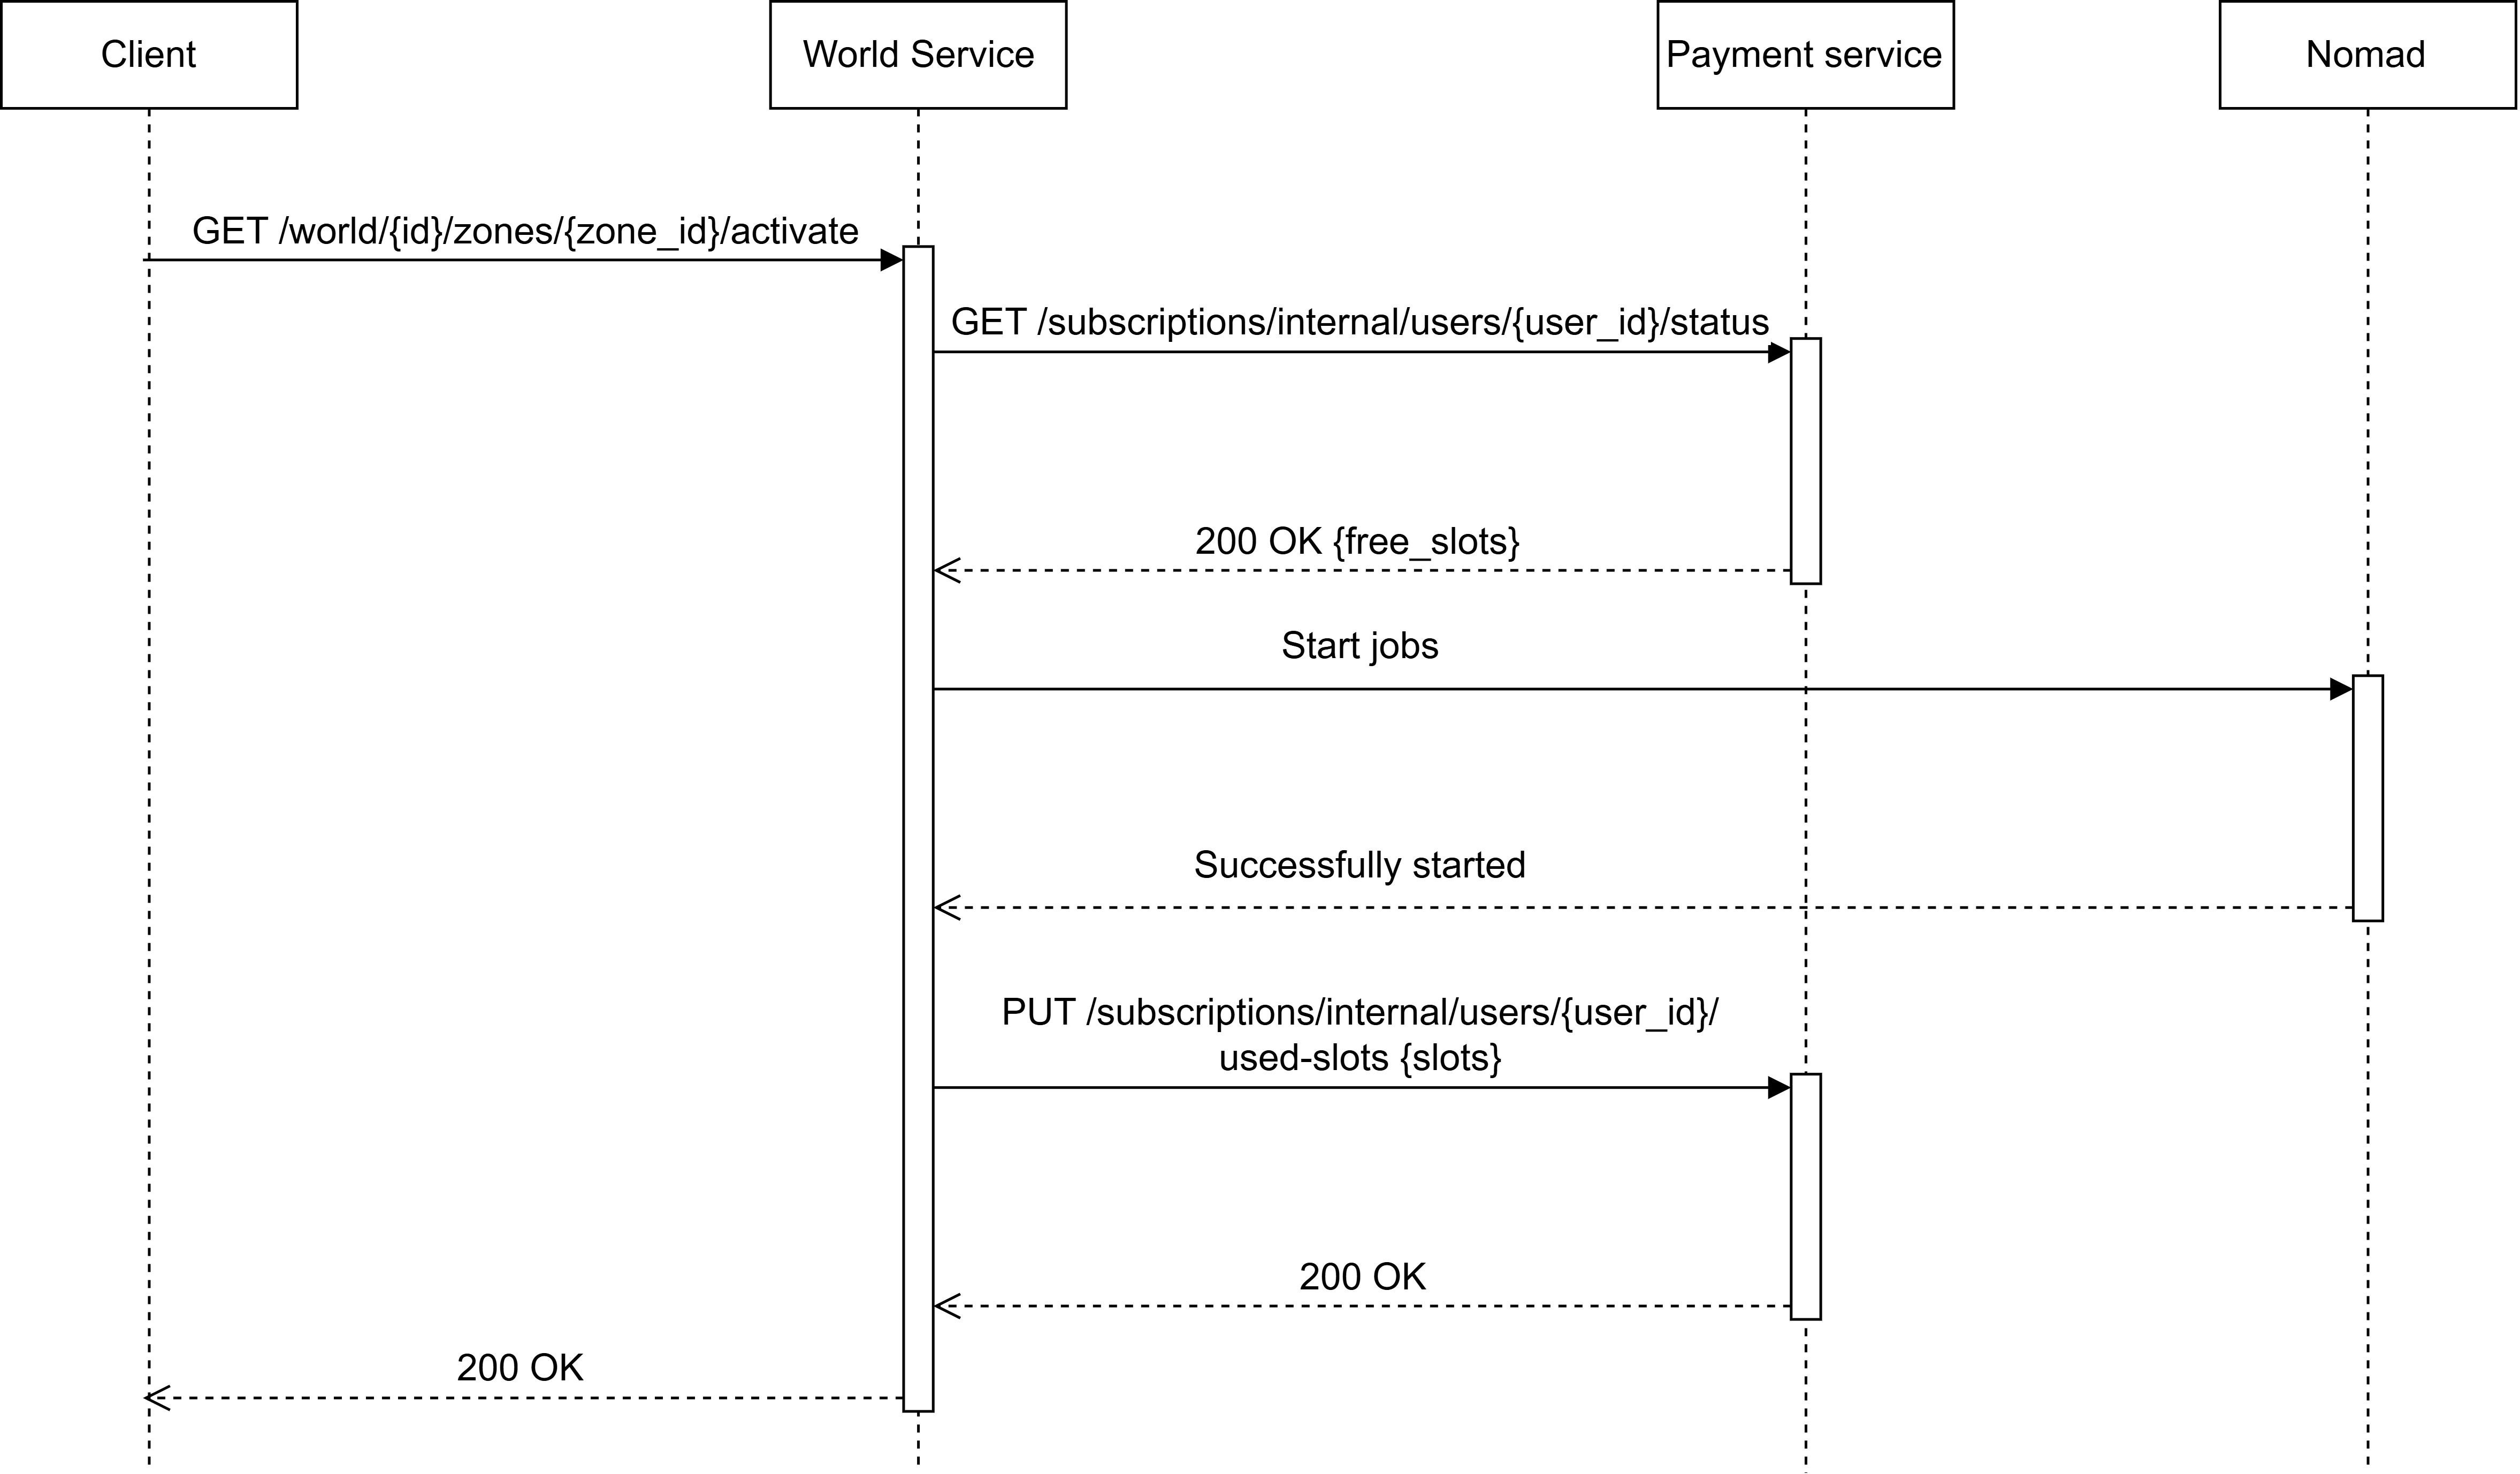
\includegraphics[width=\textwidth]{img/09-technical-details/core-service/world-service-case-2.jpg}
    \caption{Diagrama de secuencia de la actualización de los servidores.}    \label{fig:world-service-case-2}
\end{figure}

Los propios servidores de juego reportan periódicamente su estado al \textit{core service}. Cada 2 minutos
envían el recuento de jugadores activos y el tiempo promedio de sesión mediante
\texttt{POST /world/orchestrator/\{id\}/zones/\{zone\_id\}/players}, y notifican cambios en su estado de
conexión mediante \texttt{POST /world/orchestrator/\{id\}/zones/\{zone\_id\}/status}.
\vspace{0.25cm}

Finalmente, el \textit{endpoint} \texttt{POST /world/orchestrator/webhook/servers/update} permite actualizar todos los
servidores en ejecución ante un nuevo despliegue, por el cambio en una imagen, autenticando la petición mediante un token 
OIDC de GitHub para restringir su uso a los flujos de integración continua.
\vspace{0.25cm}
